%****************************************************************************%
%* DIET User's Manual description chapter file                              *%
%*                                                                          *%
%*  Author(s):                                                              *%
%*    - Philippe COMBES (Philippe.Combes@ens-lyon.fr)                       *%
%*                                                                          *%
%* $LICENSE$                                                                *%
%****************************************************************************%
%* $Id$
%* $Log$
%* Revision 1.5  2004/10/25 08:59:56  sdahan
%* add the multi-MA documentation
%*
%* Revision 1.4  2004/01/29 17:08:47  ecaron
%* Add suggestions from Frederic Desprez. Thanks !
%*
%* Revision 1.3  2004/01/21 23:23:03  ecaron
%* Add suggestions from Jean-Yves. Thanks !
%*
%* Revision 1.2  2004/01/15 23:59:31  ecaron
%* Add corrections from Holly Dail
%*
%* Revision 1.1  2003/09/09 12:38:20  pcombes
%* Reorganization of doc: UM becomes UsersManual.
%*
%* Revision 1.9  2003/06/02 13:47:05  pcombes
%* Fix footnotesize.
%*
%* Revision 1.8  2003/05/15 14:17:58  pcombes
%* UM 0.7
%*
%* Revision 1.5  2003/01/22 17:34:53  pcombes
%* User Manual, v. 0.6.4
%*
%* Revision 1.4  2003/01/21 12:17:02  pcombes
%* Update UM to API 0.6.3, and "hide" data structures.
%*
%* Revision 1.3  2003/01/13 12:09:00  pcombes
%* UM: client part complete for users's day ...
%****************************************************************************%

\chapter{A DIET platform}
\label{ch:description}

DIET is built upon the \emph{Server Daemons}. The scheduler is
scattered across a hierarchy of \emph{Local Agents} and \emph{Master
  Agents}. NWS~\cite{WSH99} sensors are placed on every node of the
hierarchy to collect resource availabilities, which are used by an
application-centric performance prediction tool called FAST
\cite{Qui02}.  Figure~\ref{fig:platform} shows the hierarchical
organization of DIET.

\begin{figure}[htb]
 \begin{center}
  \resizebox{.7\linewidth}{!}{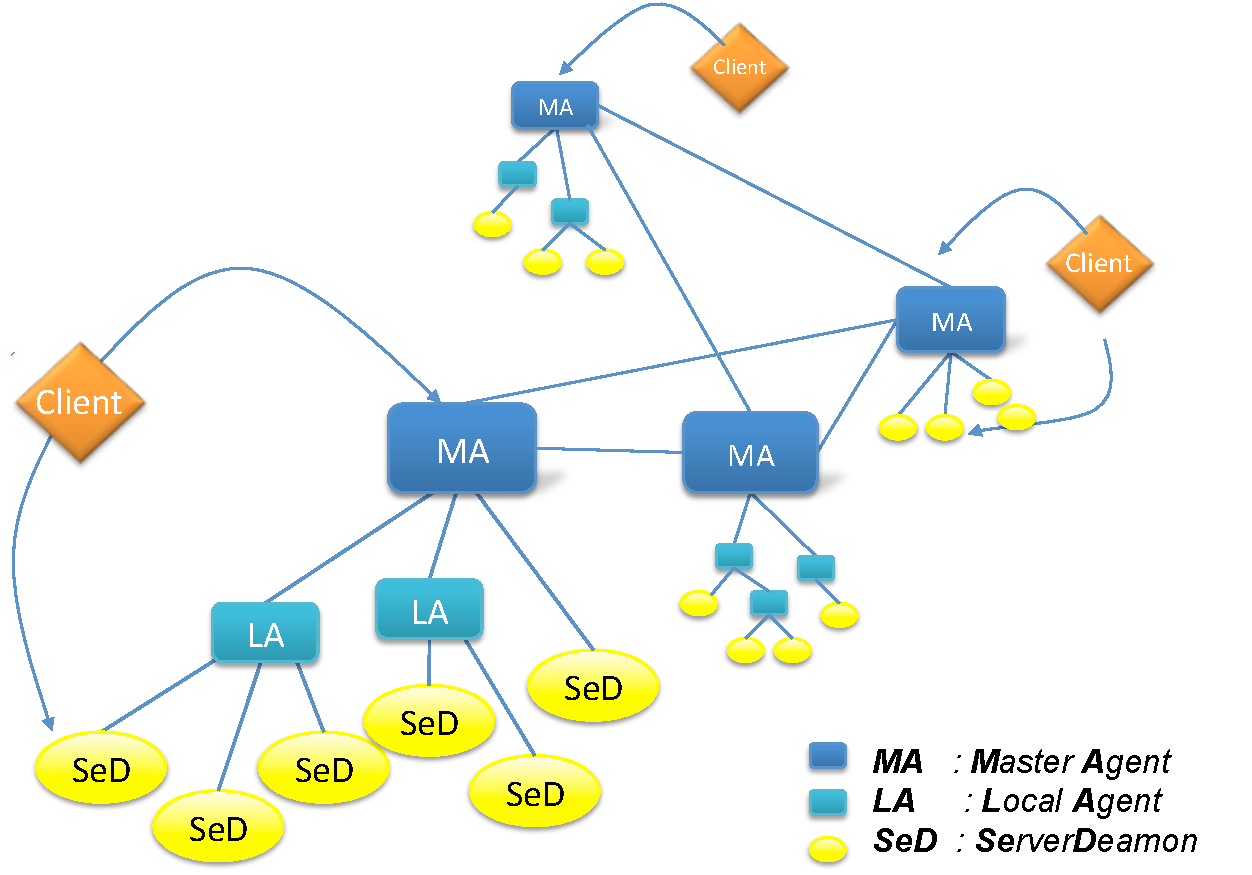
\includegraphics{fig/global_platform.eps}}
  \label{fig:platform}
  \caption{A hierarchy of DIET agents}
 \end{center}
\end{figure}

%====[ DIET components ]=======================================================
\section{DIET components}
\label{sec:components}

The different components of our software architecture are the following:      

\begin{description}
%....[ Client ]................................................................
\item \textbf{Client}\\
  A client is an application which uses DIET to solve problems.  Many types of clients are able to connect to DIET from a web page, a PSE such as
  Matlab or \sci, or from a compiled program.
%....[ Master Agent (MA) ].....................................................
\item \textbf{Master Agent (MA)}\\
  An MA receives computation requests from clients. These requests
  refer to some DIET problems listed on a reference web
  page~\footnote{http://graal.ens-lyon.fr/DIET/diet\_services.html}.
  Then the MA collects computation abilities from the servers and
  chooses the best one. The reference of the chosen server is returned
  to the client. A client can be connected to an MA by a specific name
  server or a web
  page~\footnote{http://graal.ens-lyon.fr/DIET/diet\_access.html} which
  stores the various MA locations.

%....[ Local Agent (LA) ]......................................................
\item \textbf{Local Agent (LA)}\\
  An LA aims at transmitting requests and information between MAs and
  servers.  The information stored on an LA is the list of the
  requests being processed and performance of all servers in its
  subtree that can solve a given problem. Depending on the underlying
  network topology, a hierarchy of LAs may be deployed between an MA
  and the servers. Of course, the function of an LA is to do a partial
  scheduling on its subtree, which reduces the job of the MA.

%....[ Server Daemon (SeD) ]...................................................
\item \textbf{Server Daemon (SeD)}\\
  A SeD encapsulates a computational server. For instance it can be
  located on the entry point of a parallel computer. The information
  stored on a SeD is a list of the data available on its server (with
  their distribution and the way to access them), the list of problems
  that can be solved on it, and all information concerning its load
  (memory available, number of resources available, \ldots). A SeD
  declares the problems it can solve to its parent LA.  An SeD can give
  performance predictions for a given problem thanks to the module
  FAST, described in the next section.

\end{description}

%\begin{figure}[htb]
% \begin{center}
%  \resizebox{.6\linewidth}{!}{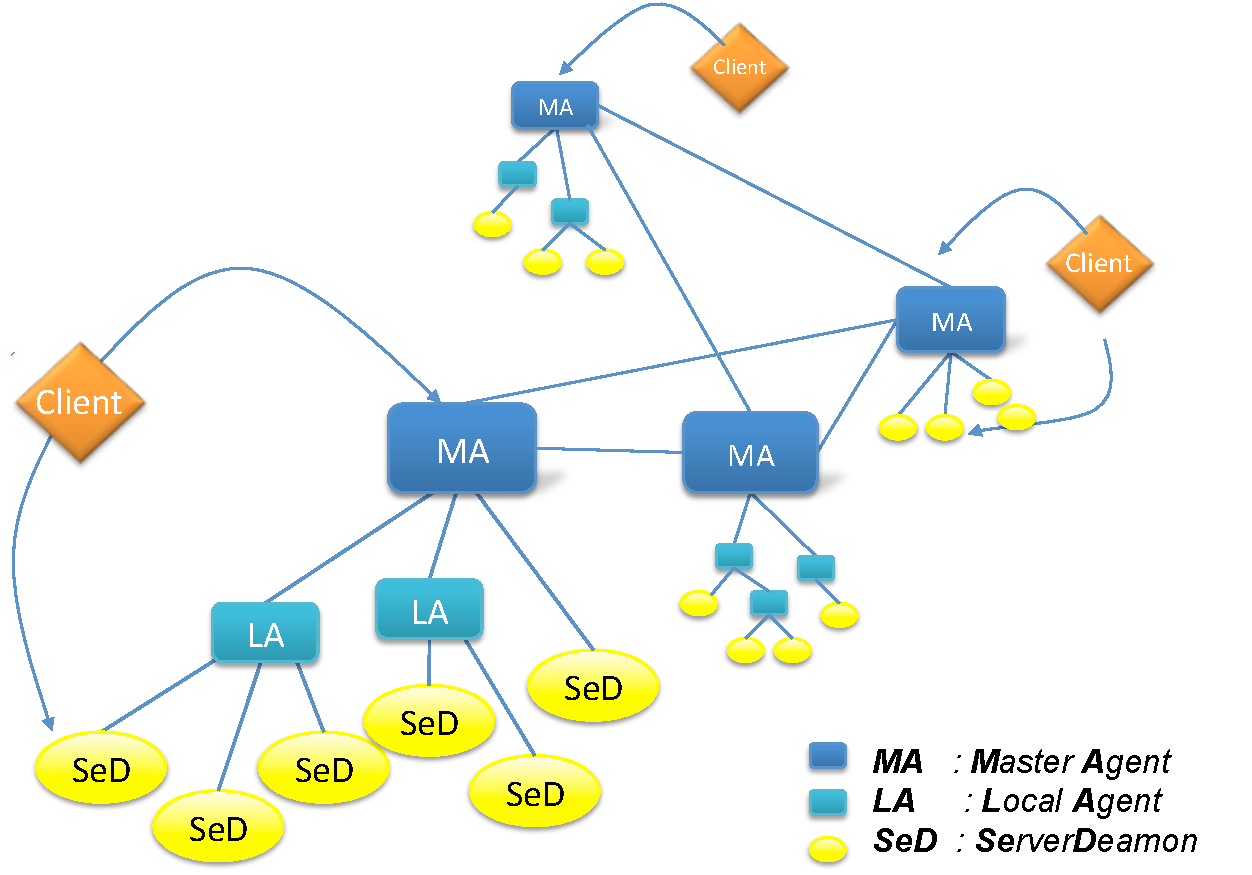
\includegraphics{fig/global_platform.eps}}
%  \label{fig:platform}
%  \caption{A hierarchy of DIET agents}
% \end{center}
%\end{figure}


%====[ FAST: FAST AGENT'S SYSTEM TIMER ]=======================================
\section{FAST: Fast Agent's System Timer}
\label{sec:FAST}

FAST \cite{Qui02} is a tool for dynamic performance forecasting in a
Grid environment. As shown in Figure~\ref{fig:fast-overview}, FAST is
composed of several layers and relies on low-level software. First it
uses a network and CPU monitoring software to handle dynamically
changing resources, like workload or bandwidth.  FAST uses the Network
Weather Service (NWS)~\cite{WSH99}, a distributed system that
periodically monitors and dynamically forecasts the performance of
various network and computational resources. The resource
availabilities acquisition module of FAST uses and enhances NWS.
Indeed, if there is no direct NWS monitoring between two machines,
FAST automatically searches for the shortest path between them in the
graph of monitored links. It estimates the bandwidth as the minimum of
those in the path and the latency as the sum of those measured. This
allows for the availability of more predictions when DIET is deployed
over a hierarchical network.

\begin{figure}[htb]
  \begin{center}
    \resizebox{.75\linewidth}{!}{\includegraphics{fig/FAST.eps}}
    \caption{FAST overview}
    \label{fig:fast-overview}
  \end{center}
\end{figure}

In addition to the system availabilities, FAST can also forecast the
time and space needs of computational routines, depending on both the
parameter set and the machine where the computation would take place.
For this, FAST benchmarks the routines at installation time on each
machine for a representative set of parameters. After polynomial data
fitting, the results are stored in an LDAP tree.  The user API of FAST
is composed of a small set of functions that combine resource
availabilities and routine needs from low-level software to produce
ready-to-use values.  These results can be combined into analytical
models by the parallel extension~\cite{CS02} to forecast execution
times of parallel routines.

Thus DIET components, as any FAST client, can access information like the time
needed to move a given amount of data between two SeDs, the time to solve a
problem with a given set of computational resources managed by a SeD, or the
combination of these two quantities.\\

For more details about FAST, please read the FAST Reference Manual~\footnote{\url{http://graal.ens-lyon.fr/FAST/docs}}.


%====[ CORBA ]=================================================================
\section{Communications inner to the platform}
\label{sec:CORBA}

NES environments can be implemented using a classic socket
communication layer.  Several problems to this approach have been
pointed out such as the lack of portability or the limitation of
opened sockets. Our aim is to implement and deploy a distributed NES
environment that works at a wider scale. Distributed object
environments, such as \emph{Java}, \emph{DCOM} or CORBA have proven to
be a good base for building applications that manage access to
distributed services. They not only provide transparent communications
in heterogeneous networks, but they also offer a framework for the
large scale deployment of distributed applications. Being open and
language independent, CORBA was chosen as the communication layer in
DIET.

As recent implementations of CORBA provide communication time close to
that of sockets, CORBA is well suited to support distributed resources
and applications in a large scale Grid environment. New specialized
services can be easily published and existing services can also be
used.  Therefore, CORBA is a good choice for the
development of Grid specific services. DIET is based upon
\emph{OmniORB 3}~\cite{OMNIORB} or later, a free CORBA implementation
which provides good communication performance.


%====[ Multi-MA ]==============================================================
\section{Multi-MA}
\label{init:multima}

LA, SeD and a MA are put together to form a hierarchy. It is possible to
federate those hierarchies by connecting the MA together. when DIET is run in
multi-MA mode, the behavior of the architecture does not change, but if a SeD
that can resolved a problem is not found inside a hierarchy, the architecture
will automatically looking for a SeD inside the other hierarchies.

%====[ DIET INITIALIZATION ]===================================================
\section{DIET initialization}
\label{init}

Figure~\ref{fig:init} shows each step of the initialization of a simple Grid
system. The architecture is built in hierarchical order, each component
connecting to its parent. The MA is the first entity to be started~(1). It waits
for connections from LAs or requests from clients.

\begin{figure}[hbt]
  \begin{center}
    \resizebox{9cm}{!}{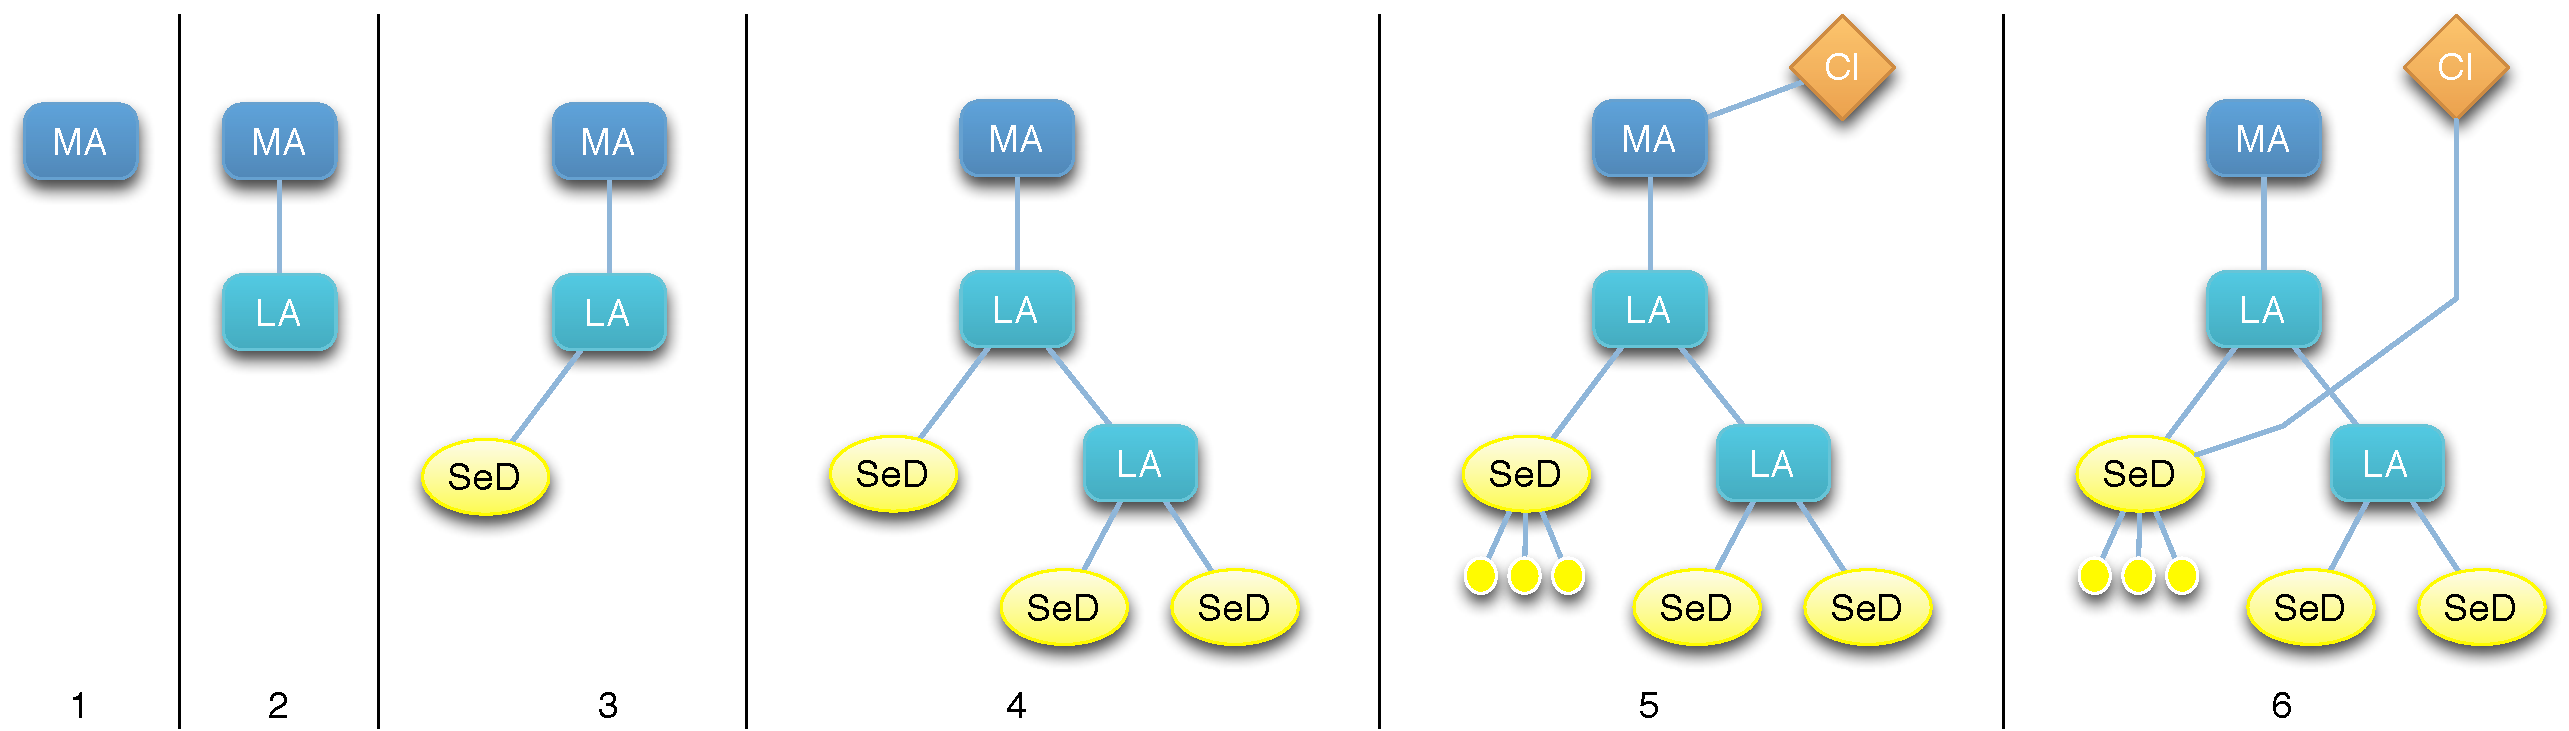
\includegraphics{fig/init.eps}}
    \caption{Initialization of a DIET system.}
    \label{fig:init}
  \end{center}
\end{figure}

Then when an LA is launched, it subscribes to the MA~(2). At this step of the
system initialization, two kinds of components can connect to the LA: an
\sed ~(3), which manages some computational resource, or another LA~(4), to add a
hierarchical level in this branch. When the \sed\ registers to an LA, it
publishes a list of the services it offers, which is forwarded to the parent
agent until the MA.
Finally, any client can access the registered resource through the platform: it
can contact an MA~(5) to get a reference to the best server available and then
directly connect to it to launch the computation.

The architecture of the hierarchy is described in configuration files and each
component transmits the local configuration to its parent. Thus, the system
administration can also be hierarchical. For instance, an MA can manage a domain
like a university, providing prioritary access to users of this domain. Then
each laboratory can run an LA, while each team of the laboratory can run some
other LAs to administrate its own servers. This hierarchical administration of
the system allows local changes in the configuration without interfering with
the whole platform.



%====[ Solving a problem ]=====================================================
\section{Solving a problem}
\label{sec:solvepb}

Assuming that the architecture described in Section
\ref{sec:components} includes several servers able to solve the same
problem, the algorithm presented below lets an MA choose among its
servers the one which will perform the computation. This decision is
made in four steps:


%%%%%%%%%%%%%%%
%% FIXME for DIET v1.1
%%%%%%%%%%%%%%%
% , and that each operand
% needed for the computation is available on one single server, the example
% presented in Figure~\ref{fig:submit_pb} considers the submission of the
% problem \texttt{F()} involving data \texttt{A} and \texttt{B}.
%\begin{figure}[hbt]
%  \begin{center}
%    \resizebox{8cm}{!}{\includegraphics{fig/submit_pb.eps}}
%    \caption{Problem submission example}
%    \label{fig:submit_pb}
%  \end{center}
%\end{figure}
%%%%%%%%%%%%%%%


\begin{itemize}
\item the MA propagates the client request through its subtrees down to the
  capable servers~; actually, each agent only knows which among its children manage
  the service, and it forwards the client request to them only~;
\item each server that can satisfy the request calls FAST to estimate the
  computation time necessary to process the request, and sends this
  estimation back to its ``parent'' (the LA)~;
\item each LA of the tree that receives one or more positive answers from its
  children sorts the servers and forwards their answers to the MA through the
  hierarchy~;
\item once the MA has collected all the answers from its direct children, it
  chooses a pool of fast servers and sends their references to the client.
\end{itemize}

If the multi-MA option is enabled and no server is found, then the MA
propagates the client request to the other MA which follow at their turn the
same pattern.

%%%%%%%%%%%%%%%
%% FIXME:
%%  Memory aspects should be treated here.
%%%%%%%%%%%%%%%

%%%%%%%%%%%%%%%
%% FIXME for DIET v1.1
%%%%%%%%%%%%%%%
% In order to solve the problem itself, the client connects to one of
% the servers chosen: it sends its local data and specifies if the
% results should be kept in-place for further computation or if they
% should be brought back. The transfer of persistent operands is
% performed at this stage.
%%%%%%%%%%%%%%%
